\documentclass{article}
\usepackage{wvwcmath}

\pgfplotsset{compat=newest}
\usetikzlibrary{%
  angles,
  arrows,
  backgrounds,
  calc,
  decorations.pathmorphing,
  decorations.markings,
  decorations.pathreplacing,
  graphs,
  graphs.standard,
  intersections,
  patterns,
  positioning,
  quotes,
  shapes.geometric,
  }
\usepgfplotslibrary{%
  fillbetween,
  colorbrewer
  }

\definecolor{darkgreen}{rgb}{0.125,0.5,0.169}

% Functions for point mass examples in 7.6
\pgfmathdeclarefunction{curvei}{1}{%
\pgfmathparse{0.05*#1*(#1-7)*(#1-12)}%
}
\pgfmathdeclarefunction{curveii}{1}{%
\pgfmathparse{-0.03*(#1)*(#1-6)*(#1-18)}%
}

% my axis/plot settings; partially inspired by ORCCA calc manual
\pgfplotsset{
  % cycle list/Set1,
  colormap/Set1,
  % define a style that incorporates the `cycle list`
  MyCycleList cycle list/.style={
    cycle multiindex* list={
    linestyles*\nextlist
    mark=none\nextlist
    Set1%
    },
  },
  myplot/.style={% primary style for curves
    mark=none,
    line width=1pt,
    <->,
    smooth,
    samples=100,
    },
  myaxis/.style={% primary style for axes
    view={120}{30},
    % cycle list name=Set1,
    % cycle list name=linestyles*,
    MyCycleList cycle list,
    axis lines=center,
    axis line style={shorten <=-10pt, shorten >=-10pt, latex-latex},
    % axis line style = {latex-latex},
    axis equal image,
    xlabel={$x$}, xlabel style={at=(current axis.right of origin), anchor=west, xshift=10pt},
    ylabel={$y$}, ylabel style={at=(current axis.above origin), anchor=south, yshift=10pt},
    xmin = -7, xmax = 7,
    ymin = -7, ymax = 7,
    grid = both,
    grid style={line width=.1pt, draw=gray!30},
    major grid style={line width=.2pt,draw=gray!60},
    % grid = minor,
    % grid=major,
    % grid style = {solid,gray!40},
    % minor xtick = {-7,-6,...,7},
    % minor ytick = {-7,-6,...,7},
    xtick={\pgfkeysvalueof{/pgfplots/xmin},...,\pgfkeysvalueof{/pgfplots/xmax}},
    ytick={\pgfkeysvalueof{/pgfplots/ymin},...,\pgfkeysvalueof{/pgfplots/ymax}},
    minor tick num=1,
    tick label style={font=\footnotesize},
    scale only axis,  % only scale axes when specifying height/width
    legend cell align=left,
    vector/.style={-stealth,blue,very thick}
    , 
    vector guide/.style={dashed,red,thick}
    },
  numberline/.style={% style for drawing numberline
    axis x line = center,
    axis y line = none,
    axis line style={shorten >=-10pt, shorten <=-10pt, <->},
    xlabel={$x$}, xlabel style={at=(current axis.right of origin), anchor=west, xshift=10pt},
    ymin=0,
    ymax=0},
  mypolarplot/.style={%PGFPlots polaraxis settings
    clip=false, % needed for double line (last \addplot command)
    domain=0:360, % plot full cycle
    samples=180, % number of samples; can be locally adjusted
    grid=both, % display major and minor grids
    major grid style={gray!70}, 
    minor grid style={gray!20}, 
    minor x tick num=3, % 3 minor x ticks between majors
    minor y tick num=1, % 1 minor y tick between majors
    xtick={0,30,45,60,90,120,135,150,180,210,225,240,270,300,315,330},
    xticklabels={%
      $0$,
      $\frac{\pi}{6}$,
      $\frac{ \pi}{4}$,
      $\frac{\pi}{3}$,
      $\frac{ \pi}{2}$,
      $\frac{2\pi}{3}$,
      $\frac{3\pi}{4}$,
      $\frac{5\pi}{6}$,
      $\pi$,
      $\frac{7\pi}{6}$,
      $\frac{5\pi}{4}$,
      $\frac{4\pi}{3}$,
      $\frac{3\pi}{2}$,
      $\frac{5\pi}{3}$,
      $\frac{7\pi}{4}$,
      $\frac{11\pi}{6}$
    },
    yticklabel style={anchor=north}, % move label position
    },
  }

% Make it easier to display multiple pictures
\pgfplotsset{width=5cm}

\tikzset{%
  jumpdot/.style={mark=*,solid},
  excl/.append style={jumpdot,fill=white},
  incl/.append style={jumpdot,fill=black},
  }

\begin{document}
%==============================%
%           Calculus           %
%==============================%
\section{Calculus} % (fold)
\label{sec:calculus}

  \subsection{Chapter 9}
  %===============================%
  %           CHAPTER 9           %
  %===============================%
    \href{https://j-oldroyd.github.io/wvwc-calculus/output/html/section-power-series.html#example-convergence-of-a-power-series-ratio-test}{Example 9.5.2: Convergence of a power series using the Ratio Test}
    \begin{center}
      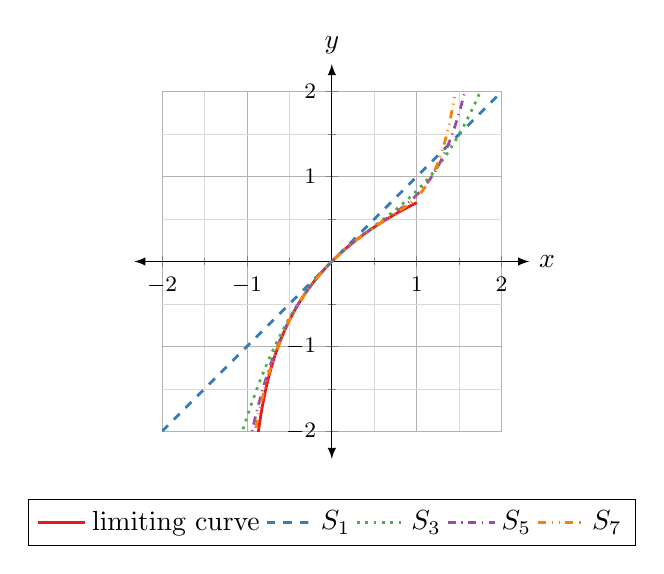
\begin{tikzpicture}
        \begin{axis}[
          myaxis,
          xmin=-2,xmax=2,
          ymin=-2,ymax=2,
          % legend style={at={(axis cs:1,-1)}, anchor={west}},
          legend style={at={(0.5,-0.2)}, anchor={north},legend columns=-1},
          ]
          \addplot+[myplot,-,domain=-1:1]{ln(1+x)};
          \addlegendentry{limiting curve}
          \addplot+[myplot,-,domain=-2:2]{x};
          \addlegendentry{$S_1$};
          \addplot+[myplot,-,domain=-2:2]{x-x^2/2+x^3/3};
          \addlegendentry{$S_3$};
          \addplot+[myplot,-,domain=-2:2]{x-x^2/2+x^3/3-x^4/4+x^5/5};
          \addlegendentry{$S_5$};
          \addplot+[myplot,-,domain=-2:2]{x-x^2/2+x^3/3-x^4/4+x^5/5-x^6/6+x^7/7};
          \addlegendentry{$S_7$};
        \end{axis}
      \end{tikzpicture}
    \end{center}

    \href{https://j-oldroyd.github.io/wvwc-calculus/output/html/section-representing-functions-as-power-series.html#example-finding-power-series-by-completing-the-square-and-partial-fractions}{Example 9.6.3: Finding power series by completing the square and partial fractions}
    \begin{center}
      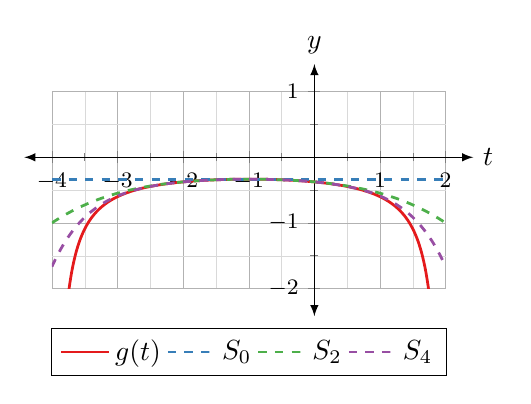
\begin{tikzpicture}
        \begin{axis}[
          myaxis,
          xlabel={$t$},
          xmin=-4,xmax=2,
          ymin=-2,ymax=1,
          domain=-4:2, restrict y to domain=-10:10,
          % legend style={at={(axis cs:1,1)}, anchor={west}},
          % code below makes use of relative axis coordinates which
          % range from 0,1 along both axes
          legend style={at={(0.5,-0.2)}, anchor={north},legend columns=-1},
          % legend pos = outer north east,
          % legend columns=1,
          ]
          \addplot+[myplot,-,domain=-4:2]{3/(x^2+2*x-8)};
          \addlegendentry{$g(t)$}
          \addplot+[myplot,dashed,-,]{-1/3};
          \addlegendentry{$S_0$};
          \addplot+[myplot,dashed,-,]{-1/3 - (x+1)^2/27 - (x+1)^4/243};
          \addlegendentry{$S_2$};
          \addplot+[myplot,dashed,-]{-1/19683*x^8 - 8/19683*x^7 - 37/19683*x^6 - 110/19683*x^5 - 286/19683*x^4 - 560/19683*x^3 - 1378/19683*x^2 - 1844/19683*x - 7381/19683};
          \addlegendentry{$S_4$};
        \end{axis}
      \end{tikzpicture}
      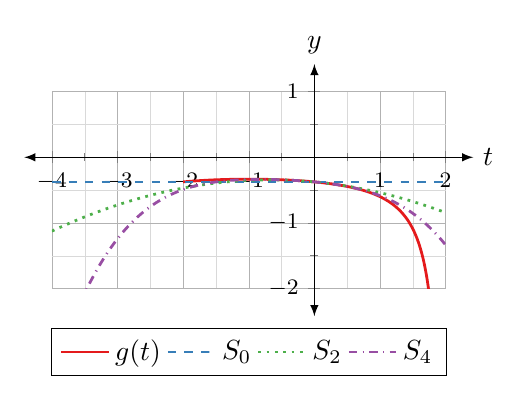
\begin{tikzpicture}
        \begin{axis}[
          myaxis,
          xlabel={$t$},
          xmin=-4,xmax=2,
          ymin=-2,ymax=1,
          domain=-4:2, restrict y to domain=-10:10,
          % code below makes use of relative axis coordinates which
          % range from 0,1 along both axes
          legend style={at={(0.5,-0.2)}, anchor={north},legend columns=-1},
          % legend columns=4,
          % legend pos = outer north east,
          ]
          \addplot+[myplot,-,domain=-2:2]{3/(x^2+2*x-8)};
          \addlegendentry{$g(t)$}
          \addplot+[myplot,-]{-3/8};
          \addlegendentry{$S_0$};
          \addplot+[myplot,-]{-9/128*x^2 - 3/32*x - 3/8};
          \addlegendentry{$S_2$};
          \addplot+[myplot,-]{-33/2048*x^4 - 15/512*x^3 - 9/128*x^2 - 3/32*x - 3/8};
          \addlegendentry{$S_4$};
        \end{axis}
      \end{tikzpicture}
    \end{center}

  \subsection{Chapter 10}
  %================================%
  %           CHAPTER 10           %
  %================================%
    \href{Figure 10.1.1}{https://j-oldroyd.github.io/wvwc-calculus/output/html/section-parametric-equations.html\#figure-parametric-parabola}
    \begin{center}
      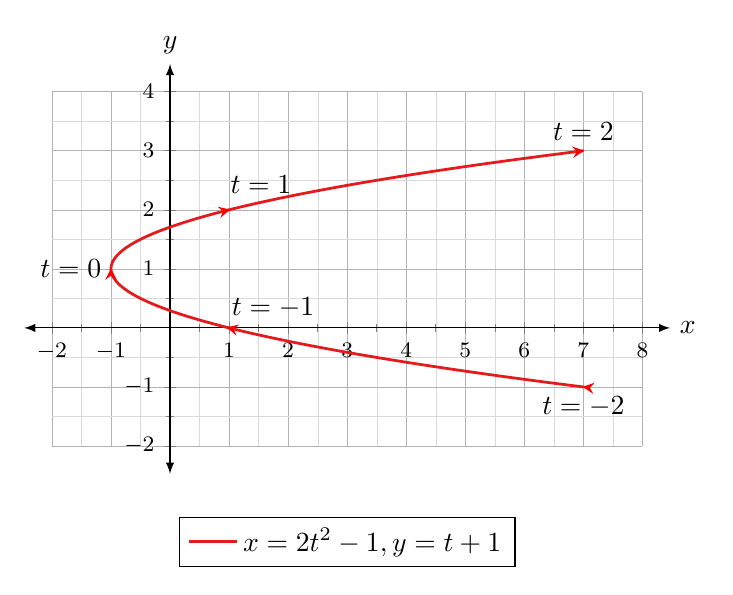
\begin{tikzpicture}
        \begin{axis}[
        myaxis,
        scale only axis,
        scale=1.5,
        xmin=-2, xmax=8,
        ymin=-2, ymax=4,
        legend style={at={(0.5,-0.2)}, anchor={north},legend columns=-1},
        clip=false,
        ]
        \addplot+[myplot,variable=\t,domain=-2:2,-] ({2*t^2-1}, {t+1});
        \addlegendentry{$x = 2t^2-1, y=t+1$};

        \def\NORM{sqrt((2*t^2-1)^2 + (t+1)^2)}
        \addplot[thick, red,-stealth,samples=5,variable=\t, domain=-2:2, quiver={
            u=4*t/\NORM, v=1/\NORM,
            scale arrows=0.01,
        }]
        ({2*t^2-1}, {t+1});

        \coordinate (A) at (axis cs:7,-1);
        \coordinate (B) at (axis cs:1,0);
        \coordinate (C) at (axis cs:-1,1);
        \coordinate (D) at (axis cs:1,2);
        \coordinate (E) at (axis cs:7,3);


        \node[below] at (A) {$t=-2$};
        \node[above right, xshift=-2.5pt] at (B) {$t=-1$};
        \node[left] at (C) {$t=0$};
        \node[above right, yshift=2.5pt, xshift=-3pt] at (D) {$t=1$};
        \node[above] at (E) {$t=2$};
        \end{axis}
      \end{tikzpicture}
    \end{center}
% section calculus (end)

%============================================%
%           Differential Equations           %
%============================================%
\section{Differential Equations} % (fold)
\label{sec:differential_equations}
  \subsection{Chapter 6}
    \href{Example 6.3.3: Inverse transform involving an exponential}{https://j-oldroyd.github.io/wvwc-differential-equations/output/html/section-unit-step-functions-and-time-shifting.html\#example-inverse-transform-involving-an-exponential}
    \begin{center}
      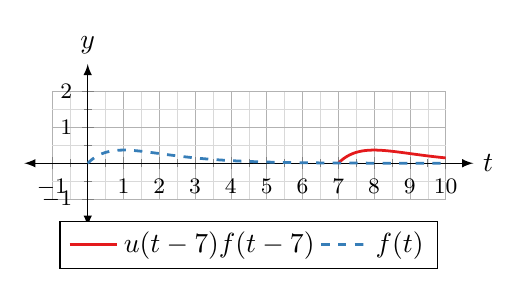
\begin{tikzpicture}
        \begin{axis}[
          myaxis,
          xmin=-1, xmax=10,
          ymin=-1, ymax=2,
          xlabel={$t$},
          % legend style={at={(axis cs:1,-1)}, anchor={west}},
          legend style={at={(0.5,-0.2)}, anchor={north},legend columns=-1},
          ]
          \addplot+[myplot,-,domain=7:10]{(x-7)*exp(7-x)};
          \addlegendentry{$u(t-7)f(t-7)$};
          \addplot+[myplot,-,domain=0:10]{x*exp(-x)};
          \addlegendentry{$f(t)$};
        \end{axis}
      \end{tikzpicture}
    \end{center}

    \subsection{Chapter 7}
    \begin{center}
      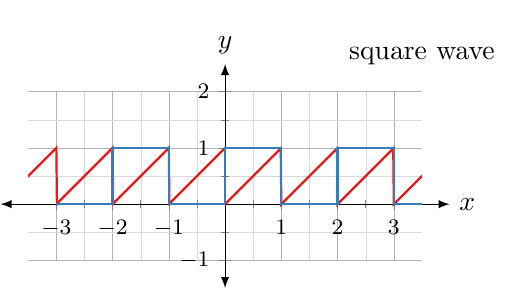
\begin{tikzpicture}
        \begin{axis}[
          myaxis,
          title={square wave},
          title style={at={(1,1)}},
          xmin=-3.5, xmax=3.5,
          ymin=-1, ymax=2,
          xtick={-3,...,3}]
          \addplot+[thick, -, samples at={0,.01,...,4},]{mod(x, 1)};
          \pgfplotsset{cycle list shift=-1};
          \addplot+[thick, -, samples at={-4,-3.99,...,0}]{mod(x, 1)+1};
          \pgfplotsset{cycle list shift=-2};
          \addplot+[thick,-,] coordinates{(0,0)(0,1)};
          \addplot+[thick,solid,-] coordinates{
            (-3,0)(-2,0)(-2,1)(-1,1)(-1,0)(0,0)(0,1)(1,1)(1,0)(2,0)(2,1)(3,1)(3,0)(4,0)
            };
        \end{axis}
      \end{tikzpicture}
    \end{center}
% section differential_equations (end)
\end{document}